\documentclass[11pt]{article}
\usepackage[margin=1in]{geometry}
\usepackage{amsmath,amssymb}
\usepackage{booktabs}
\usepackage{tabularx}
\usepackage{array}
\usepackage{graphicx}
\usepackage{float}
\usepackage{natbib}
\usepackage{hyperref}

\title{Optimizing Job Search in the ABM: Summary of the Benchmark Exercise}
\date{October 2026}

\begin{document}
\maketitle

\section{Overview}

In the baseline ABM, which extends the data-driven network model of \citet{delriochanona2021occupational}, unemployed
workers draw application effort from an empirical distribution, so search behaviour is imposed rather than chosen. We replace the effort draw with an optimizing rule and leave the rest of the model
unchanged. We then compare behavioural and non-behavioural versions of that rule inside the ABM against the baseline,
holding its calibrated parameters fixed. Table~\ref{tab:overview} lists each component and its closest counterpart in
the literature.

\begin{table}[H]
\centering
\small
\renewcommand{\arraystretch}{1.25}
\begin{tabularx}{\linewidth}{@{}>{\raggedright\arraybackslash}p{2.6cm}>{\raggedright\arraybackslash}X>{\raggedright\arraybackslash}X>{\raggedright\arraybackslash}X@{}}
\toprule
Component & Our specification & Closest literature & Main difference \\
\midrule
Application choice (all optimizing rules) & Rank found vacancies by surplus; apply while (chance of first success) $\times$
surplus $\ge \kappa w$ & Simultaneous search \citep{chade2006simultaneous}; search intensity
\citep{mortensen1977unemployment,pissarides2000equilibrium} & Discrete, myopic within the month, linear cost; exact
optimal portfolio only with equal success probabilities \\
Reservation wage & Empirical schedule declining with duration (all rules except the benchmarks) & Non-stationary search
\citep{vandenberg1990nonstationarity}; evidence in \citet{krueger2016contribution} & Not derived from the model \\
\addlinespace
\multicolumn{4}{@{}l}{\textit{Behavioural rules}} \\
Sticky beliefs (main) & Perceived success erodes with own failures, decreasing-gain update & Optimistic, slowly
revised beliefs \citep{spinnewijn2015unemployed,mueller2021job}; decreasing-gain learning \citep{evans2001learning} &
This is our own designed rule, as in Appendix A \\
Bayesian beliefs (robustness) & Beta-Bernoulli update, one failure per month & Learning from unsuccessful search
\citep{burdett1988declining,gonzalez2010equilibrium} & Static application rule; learning does not move the reservation
wage \\
\addlinespace
\multicolumn{4}{@{}l}{\textit{Non-behavioural benchmarks (no reservation wage)}} \\
Fixed beliefs & Constant perceived success probability & Stationary search intensity \citep{pissarides2000equilibrium} &
No equilibrium matching function \\
Full information & Perceived success = each occupation's realized hiring probability last month & Directed search with
multiple applications \citep{albrecht2006equilibrium,galenianos2009directed,kircher2009efficiency}; competitive search
\citep{moen1997competitive}; urn-ball hiring \citep{burdett2001pricing} & Adaptive (last month's values), not
equilibrium probabilities \\
\bottomrule
\end{tabularx}
\caption{The proposed decision rules and their closest counterparts in the literature.}
\label{tab:overview}
\end{table}

\section{Calibration strategy}

In the baseline ABM, unemployed workers draw application effort from an empirical CPS schedule. Here we replace that
draw with an optimizing rule and keep the rest of the model, including all calibrated parameters ($d_u$, $\gamma_u$,
$\theta$), unchanged. We pin down the new parameters of the decision rule outside the ABM, from micro evidence on job
search, instead of adding them to the macro calibration on the unemployment and vacancy rates. There are three reasons.
First, the unemployed rule deliberately ignores market tightness, so the two aggregate series carry almost no
information about the parameters that shape effort over an unemployment spell. Those parameters would be weakly
identified and would trade off against $d_u$ and $\gamma_u$. Second, setting parameters with a direct micro
counterpart from micro data, and leaving the remaining parameters to the macro calibration, is standard practice. It
also lets us compare the decision rules holding the calibrated economy fixed. Third, the CPS effort profile used as
an input in the baseline becomes an outcome of the optimizing model. Its model counterpart can then be checked rather
than imposed, and effort responds when the environment changes. The belief and cost parameters were chosen in a
stand-alone simulation of individual job seekers to reproduce the shape and level of the CPS effort-by-duration
profile, with reference to evidence on job seekers' beliefs \citep{mueller2021job}. This was an exploratory choice,
not a formal estimation.

\section{Behavioural decision rules}

All rules apply to unemployed workers only. Employed workers keep the baseline on-the-job search rule.

\paragraph{Common structure.}
Each month, an unemployed worker $b$ with previous wage $w_b$ and unemployment duration $\tau$ samples up to 30
vacancies from their occupational neighbourhood, as in the baseline. Vacancies paying at least the empirical
reservation wage $R_{b,\tau} = w_b\,\hat r(\tau)$, where $\hat r(\tau)$ is the estimated reservation-wage ratio by
duration, form the candidate set $\mathcal{V}_{b,t}$. Occupational similarity enters as $\tilde\rho_{ij}\in(0,1]$, the
within-row percentile of the transition weight from the worker's occupation $i$ to occupation $j$ (own occupation
$=1$). The surplus of vacancy $a$ is
\begin{equation}
\Delta V_a = (w_a - R_{b,\tau})\,\tilde\rho_{i j(a)}, \qquad a \in \mathcal{V}_{b,t},
\end{equation}
and candidates are ranked so that $\Delta V_1 \ge \Delta V_2 \ge \dots$. With a perceived per-application success
probability $p_{b,t}$ that is common across applications, the marginal benefit of the $a$-th application and the
optimal number of applications are
\begin{equation}
MB_a = (1-p_{b,t})^{a-1}\,p_{b,t}\,\Delta V_a, \qquad
A^*_{b,t} = \max\bigl\{a \le \bar A : MB_a \ge \kappa\, w_b\bigr\}, \qquad A^*_{b,t} \ge 1 .
\end{equation}
The cost is proportional to the worker's wage, so $A^*$ does not depend on the wage
level. The ceiling $\bar A = 30$ is the number of vacancies sampled. The floor of one application per month avoids an
absorbing state of zero search and can be read as a UI work-search requirement. The rules differ only in how
$p_{b,t} = \beta_{b,\tau}\,\bar p$ evolves. Beliefs are updated only on the worker's own failures, with no signal of
market tightness.

\paragraph{Sticky beliefs (main specification).}
This is equation (10) of the formalization, with no positive signals while unemployed ($h=0$):
\begin{equation}
\beta_{\tau} = \Pi_{[0,1]}\!\left(\beta_{\tau-1} - r\,e^{-\omega \tau}\right)
\;\Longrightarrow\;
\beta_{\tau} = \max\Bigl\{0,\; \beta_0 - r \textstyle\sum_{s=1}^{\tau} e^{-\omega s}\Bigr\},
\end{equation}
so beliefs erode at a decaying rate towards the floor $\beta_\infty = \beta_0 - r\,e^{-\omega}/(1-e^{-\omega})$.

\paragraph{Bayesian beliefs (robustness).}
The worker holds a Beta prior over per-application success with mean $\bar p$ and strength $N_0$, and counts one
failure per month unemployed:
\begin{equation}
\beta_{\tau} = \frac{N_0}{N_0 + \tau}.
\end{equation}
A variant that counts one failure per application was also tested. It could not reproduce the decline in effort at
long durations (fewer applications mean fewer failures, so learning stalls) and was dropped.

\begin{table}[h]
\centering
\small
\begin{tabularx}{\linewidth}{@{}lllX@{}}
\toprule
Parameter & Sticky & Bayesian & Basis \\
\midrule
$\beta_0$ & 1 & 1 (implied) & Normalization: full confidence at the start of a spell \\
$\bar p$ & 0.20 & 0.30 & Chosen to reproduce the CPS effort profile; no direct empirical counterpart \\
$\omega$ & 0.10 & -- & As in the formalization's comparative statics \\
$r$ & 0.10 & -- & Chosen for the decline after month 12. Implies $\beta_\infty \approx 0.05$ \\
$N_0$ & -- & 2 & Best fit. A weak prior, worth two months of evidence \\
$\kappa$ & 0.015 & 0.015 & Chosen to match the level of CPS effort \\
$\bar A$, $a_{\min}$ & 30, 1 & 30, 1 & Vacancies sampled; work-search requirement \\
$R_{b,\tau}$ & empirical & empirical & Baseline reservation-wage regression \\
\bottomrule
\end{tabularx}
\caption{Behavioural rules: parameter values. A sticky variant with $\bar p=0.3$, $r=0.105$ fits the CPS profile best
in the stand-alone simulation, but sets $\beta_\infty\approx 0$, so beliefs erode completely. In the ABM it performs
similarly to the main specification and is not reported.}
\end{table}

\paragraph{How realistic are these values?}
Two features need flagging. First, $\kappa = 0.015$ equals about 31 hours of wages per application
($0.015\times 2{,}080$ hours), far above measured time spent on job search \citep{krueger2010job}. Most of the cost
must therefore be non-pecuniary (effort, stress, rejection). Second, the best-fitting belief paths erode almost
completely: under the sticky rule, $\beta$ falls by about 95\% within three years, and the Bayesian prior is very
weak. \citet{mueller2021job} instead find that job seekers' beliefs are optimistic and barely revised downward. Under
both rules the decline in effort therefore comes from more belief erosion than the survey evidence suggests. However, this is calibrated to the CPS data, so our decision on this issue will depend on which source of
information we wish to follow.

\section{Non-behavioural benchmarks}

These are the counterparts of the baseline non-behavioural model. They use the same optimizing rule but switch off
both behavioural channels. There is no reservation wage, so every sampled vacancy is a candidate and the surplus is
measured from zero, $\Delta V_a = w_a\,\tilde\rho_{i j(a)}$. Neither rule depends on unemployment duration.

\paragraph{Fixed beliefs.}
Beliefs never erode ($r=0$ in the sticky rule): $p_{b,t} = \bar p$, with $MB_a$ and $A^*$ as in equation (2).

\paragraph{Full information.}
Perceived success equals each occupation's realized chance of being hired in the previous month,
\begin{equation}
p_a = \pi_{j(a),t-1}, \qquad \pi_{j,t} = \frac{1}{|\mathcal{V}_{j,t}|}\sum_{v\in \mathcal{V}_{j,t}} \frac{1}{n_{v,t}},
\end{equation}
where $n_{v,t}$ is the number of applicants to vacancy $v$. In the ABM each vacancy picks one applicant, so
$\pi_{j,t}$ is the average probability of being picked in occupation $j$. Candidates are ranked by $p_a\Delta V_a$,
and the worker applies while
\begin{equation}
MB_a = \Bigl[\textstyle\prod_{k<a}(1-p_k)\Bigr]\,p_a\,\Delta V_a \;\ge\; \kappa\, w_b .
\end{equation}
This is the only rule in which unemployed workers observe market tightness. It is a deliberate contrast to subjective
beliefs.

\begin{table}[h]
\centering
\small
\begin{tabularx}{\linewidth}{@{}lllX@{}}
\toprule
Parameter & Fixed beliefs & Full information & Basis \\
\midrule
$\bar p$ & 0.20 & -- (fallback only) & Sticky rule's belief at the start of a spell \\
$\kappa$ & 0.043 & 0.0093 & Set so mean applications per seeker equal the baseline's (5.35); refined with short ABM runs \\
Reservation wage & none & none & Behavioural channel switched off \\
\bottomrule
\end{tabularx}
\caption{Non-behavioural benchmarks: parameter values. Without a reservation wage the surplus is the whole wage, so
the same cost would buy far more search effort than in the behavioural rules. Setting $\kappa$ to match average
effort puts all rules on the same footing: each searches about as much as the data imply. The full-information benchmark
is close to a tipping point: a slightly higher cost lowers effort, raises unemployment and lowers every application's
success probability, which can push the economy into a persistent high-unemployment state.}
\end{table}

\section{Results}

All scenarios run the reference model (behavioural, cyclical on-the-job search, reservation wages) with its calibrated
parameters held fixed, 10 simulations each, 2001--2024. Only the unemployed search rule changes.

\begin{table}[H]
\centering
\small
\begin{tabular}{@{}lcccc@{}}
\toprule
 & UER RMSE & LTUER RMSE & Mean UER & Applications \\
 & 2001--2019 & 2001--2019 & 2001--2024 & per seeker \\
\midrule
Baseline (CPS effort schedule) & 0.0058 (0.0006) & 0.101 (0.004) & 0.056 & 5.35 \\
\midrule
Sticky beliefs & 0.0068 (0.0004) & 0.080 (0.005) & 0.055 & 5.66 \\
Bayesian beliefs (per month) & 0.0067 (0.0005) & 0.081 (0.006) & 0.055 & 5.50 \\
\midrule
Fixed beliefs & 0.0090 (0.0006) & 0.096 (0.004) & 0.064 & 5.51 \\
Full information & 0.0142 (0.0010) & 0.101 (0.004) & 0.068 & 5.40 \\
\bottomrule
\end{tabular}
\caption{Fit to observed series. RMSE is computed per simulation and averaged across the 10 simulations, with the
standard deviation across simulations in parentheses. The vacancy rate is exogenous and fits equally well in all
scenarios (RMSE 0.0024--0.0030).}
\end{table}

\begin{figure}[H]
\centering
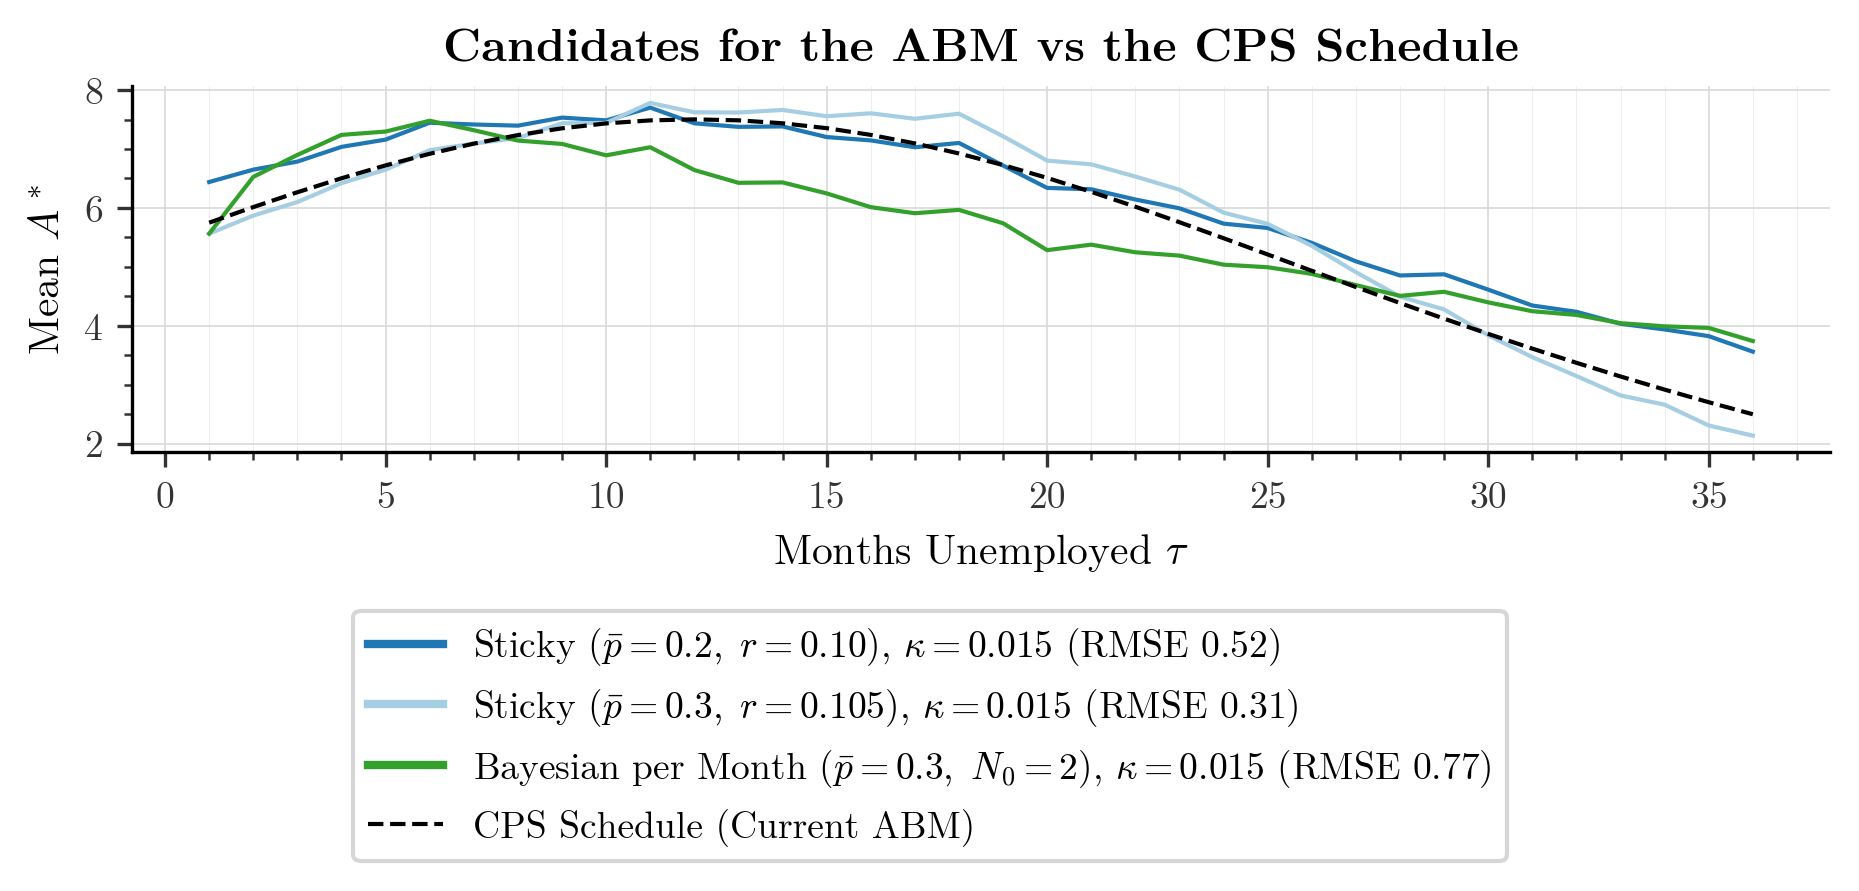
\includegraphics[width=\linewidth]{figures/opt_benchmark_best.png}
\caption{The decision rule outside the ABM: mean optimal applications by unemployment duration for simulated job
seekers who are never hired, drawing from the initial vacancy stock. RMSE is measured against the CPS schedule that the
baseline uses as input.}
\end{figure}

\begin{figure}[H]
\centering
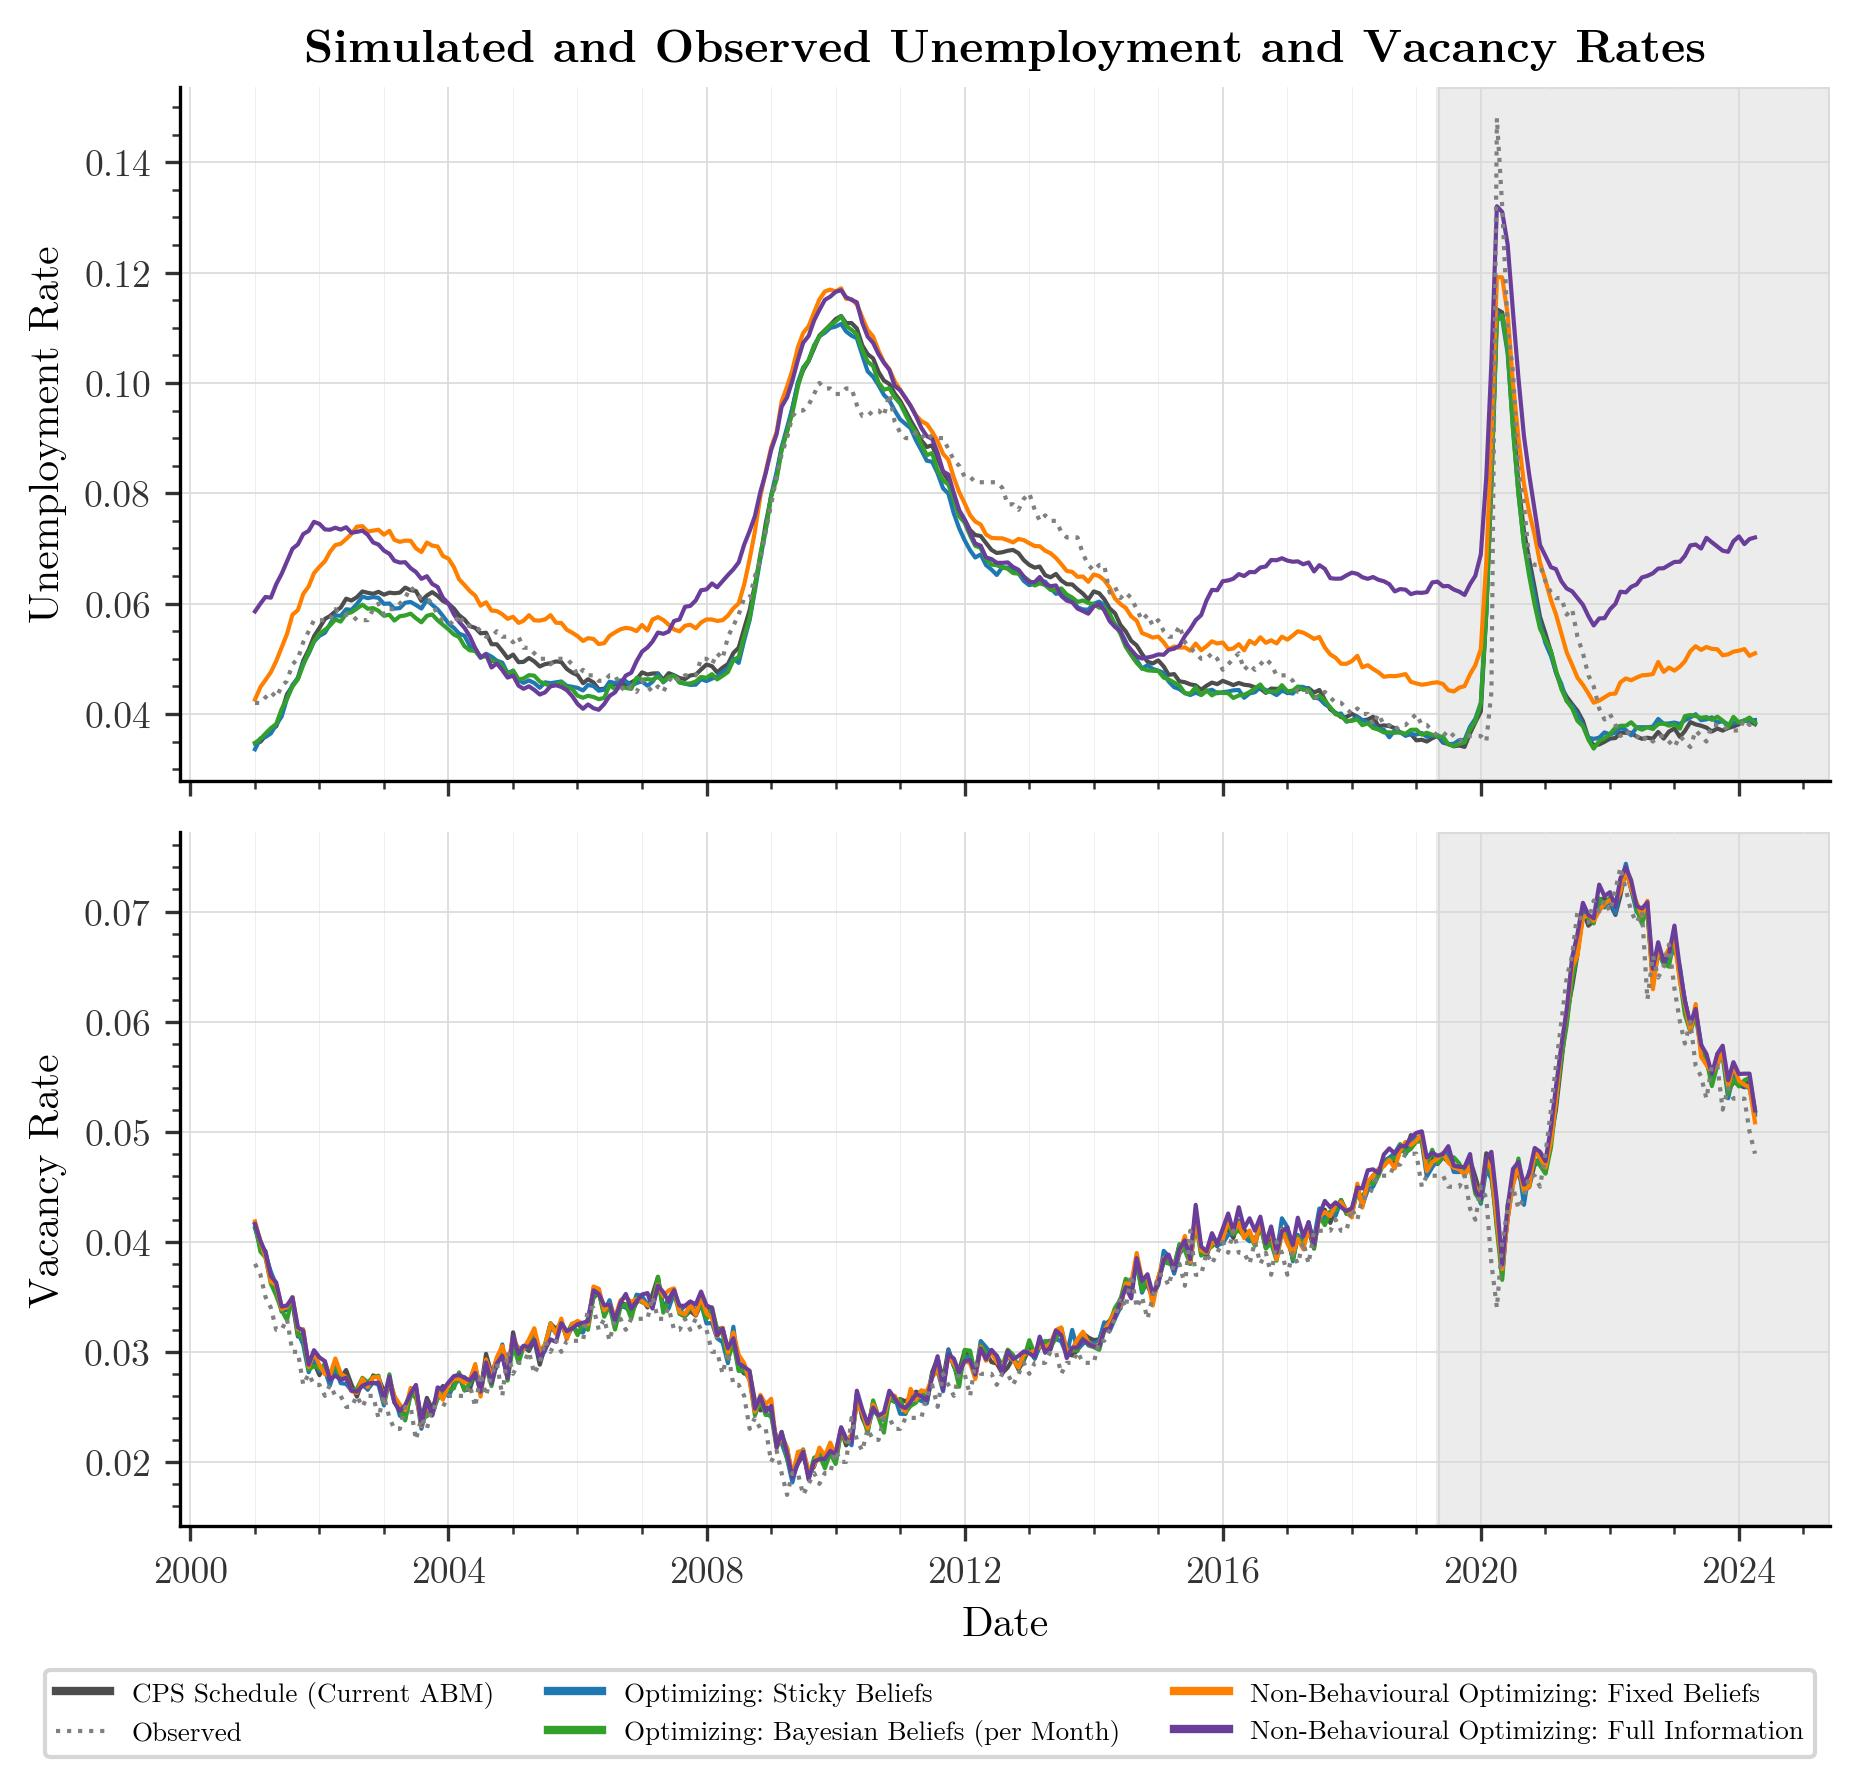
\includegraphics[width=\linewidth]{figures/uer_vac_single_panel.jpg}
\caption{Unemployment and vacancy rates. The behavioural optimizing rules track the baseline. The non-behavioural
benchmarks drift to persistently higher unemployment, even though they search as much as the baseline on average. The
shaded area is outside the calibration window.}
\end{figure}

\begin{figure}[H]
\centering
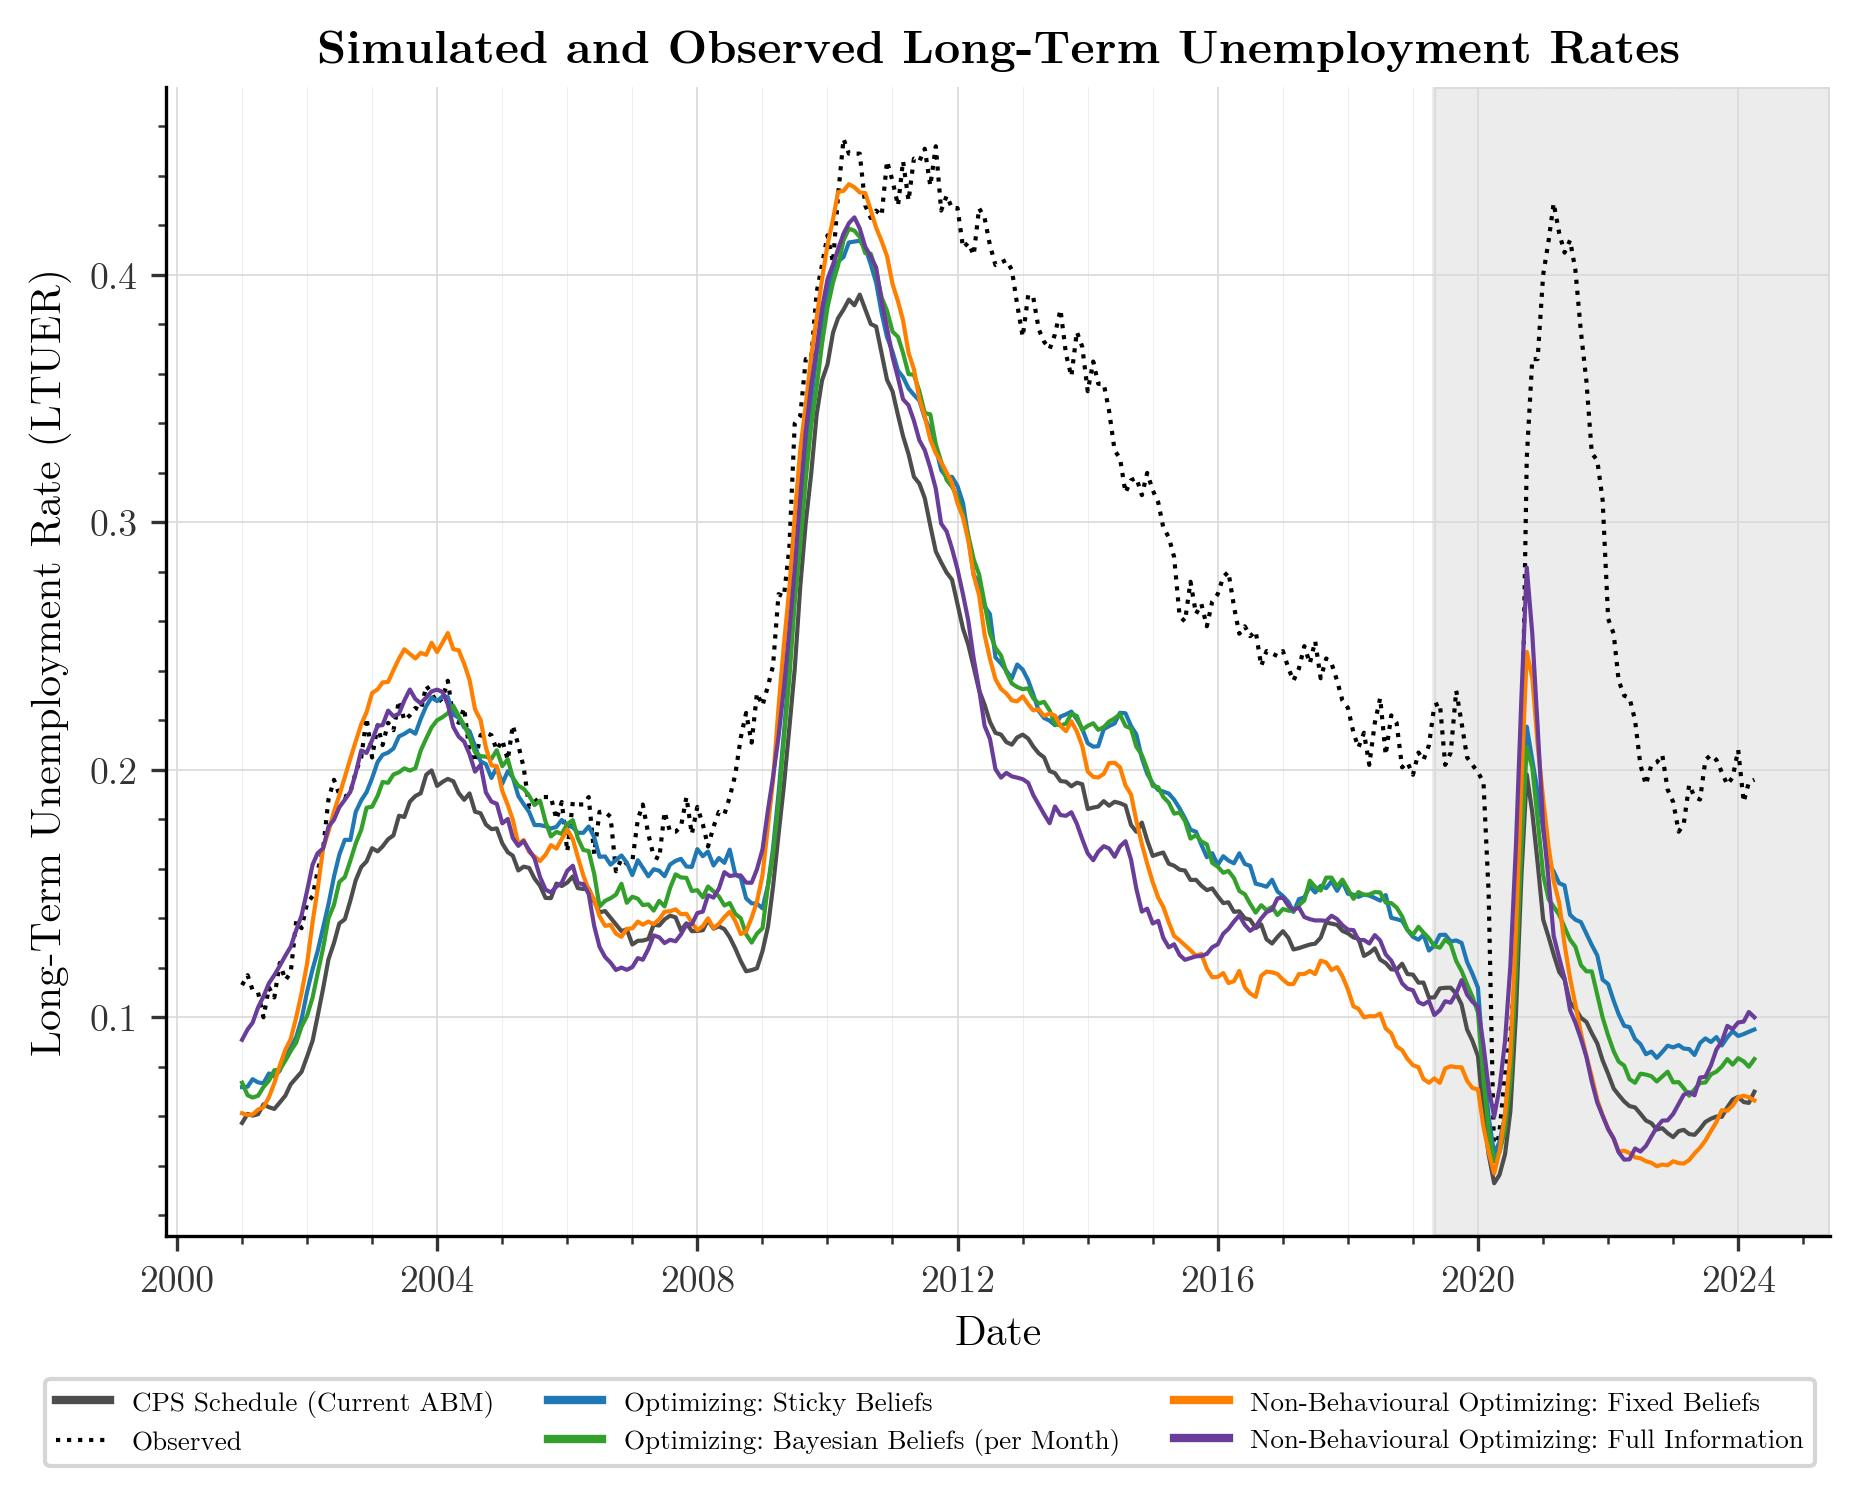
\includegraphics[width=\linewidth]{figures/ltuer_line_single_panel.jpg}
\caption{Long-term unemployment rate, simulated and observed.}
\end{figure}

\begin{figure}[H]
\centering
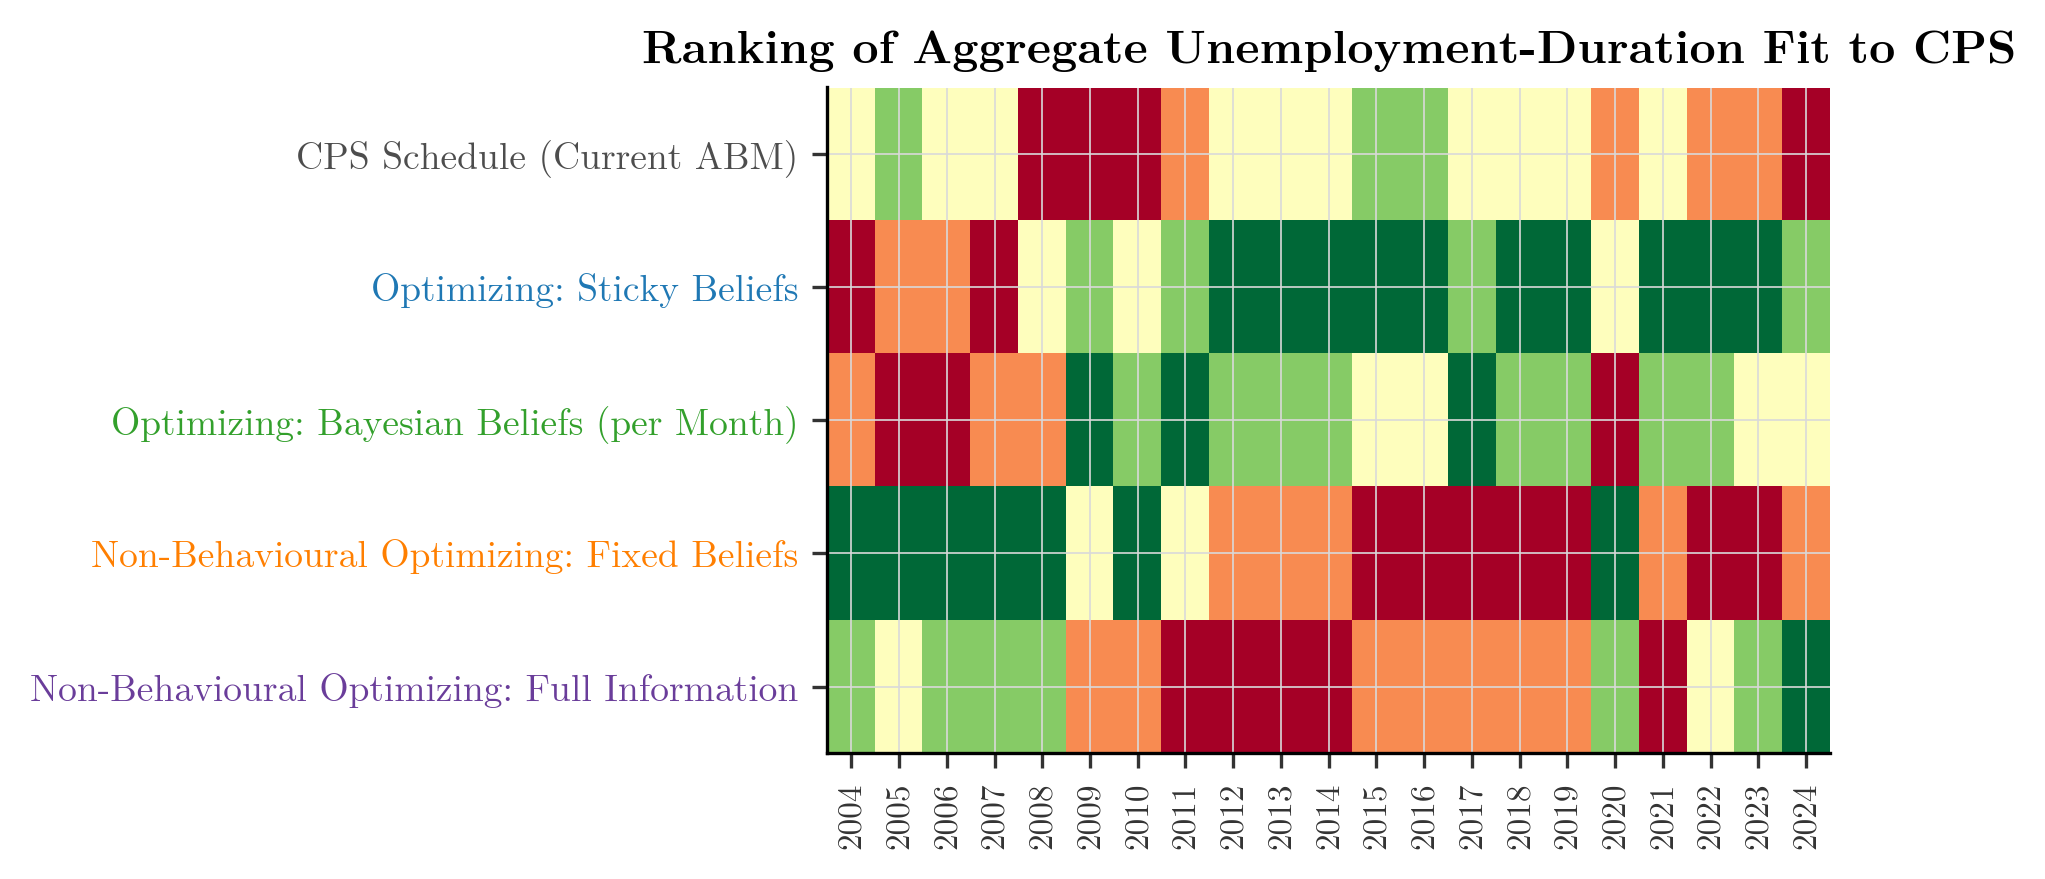
\includegraphics[width=\linewidth]{figures/duration_wasserstein_rank_heatmap.png}
\caption{Annual ranking of scenarios by the Wasserstein distance between the simulated and CPS unemployment-duration
distributions (green = closest).}
\end{figure}

\begin{figure}[H]
\centering
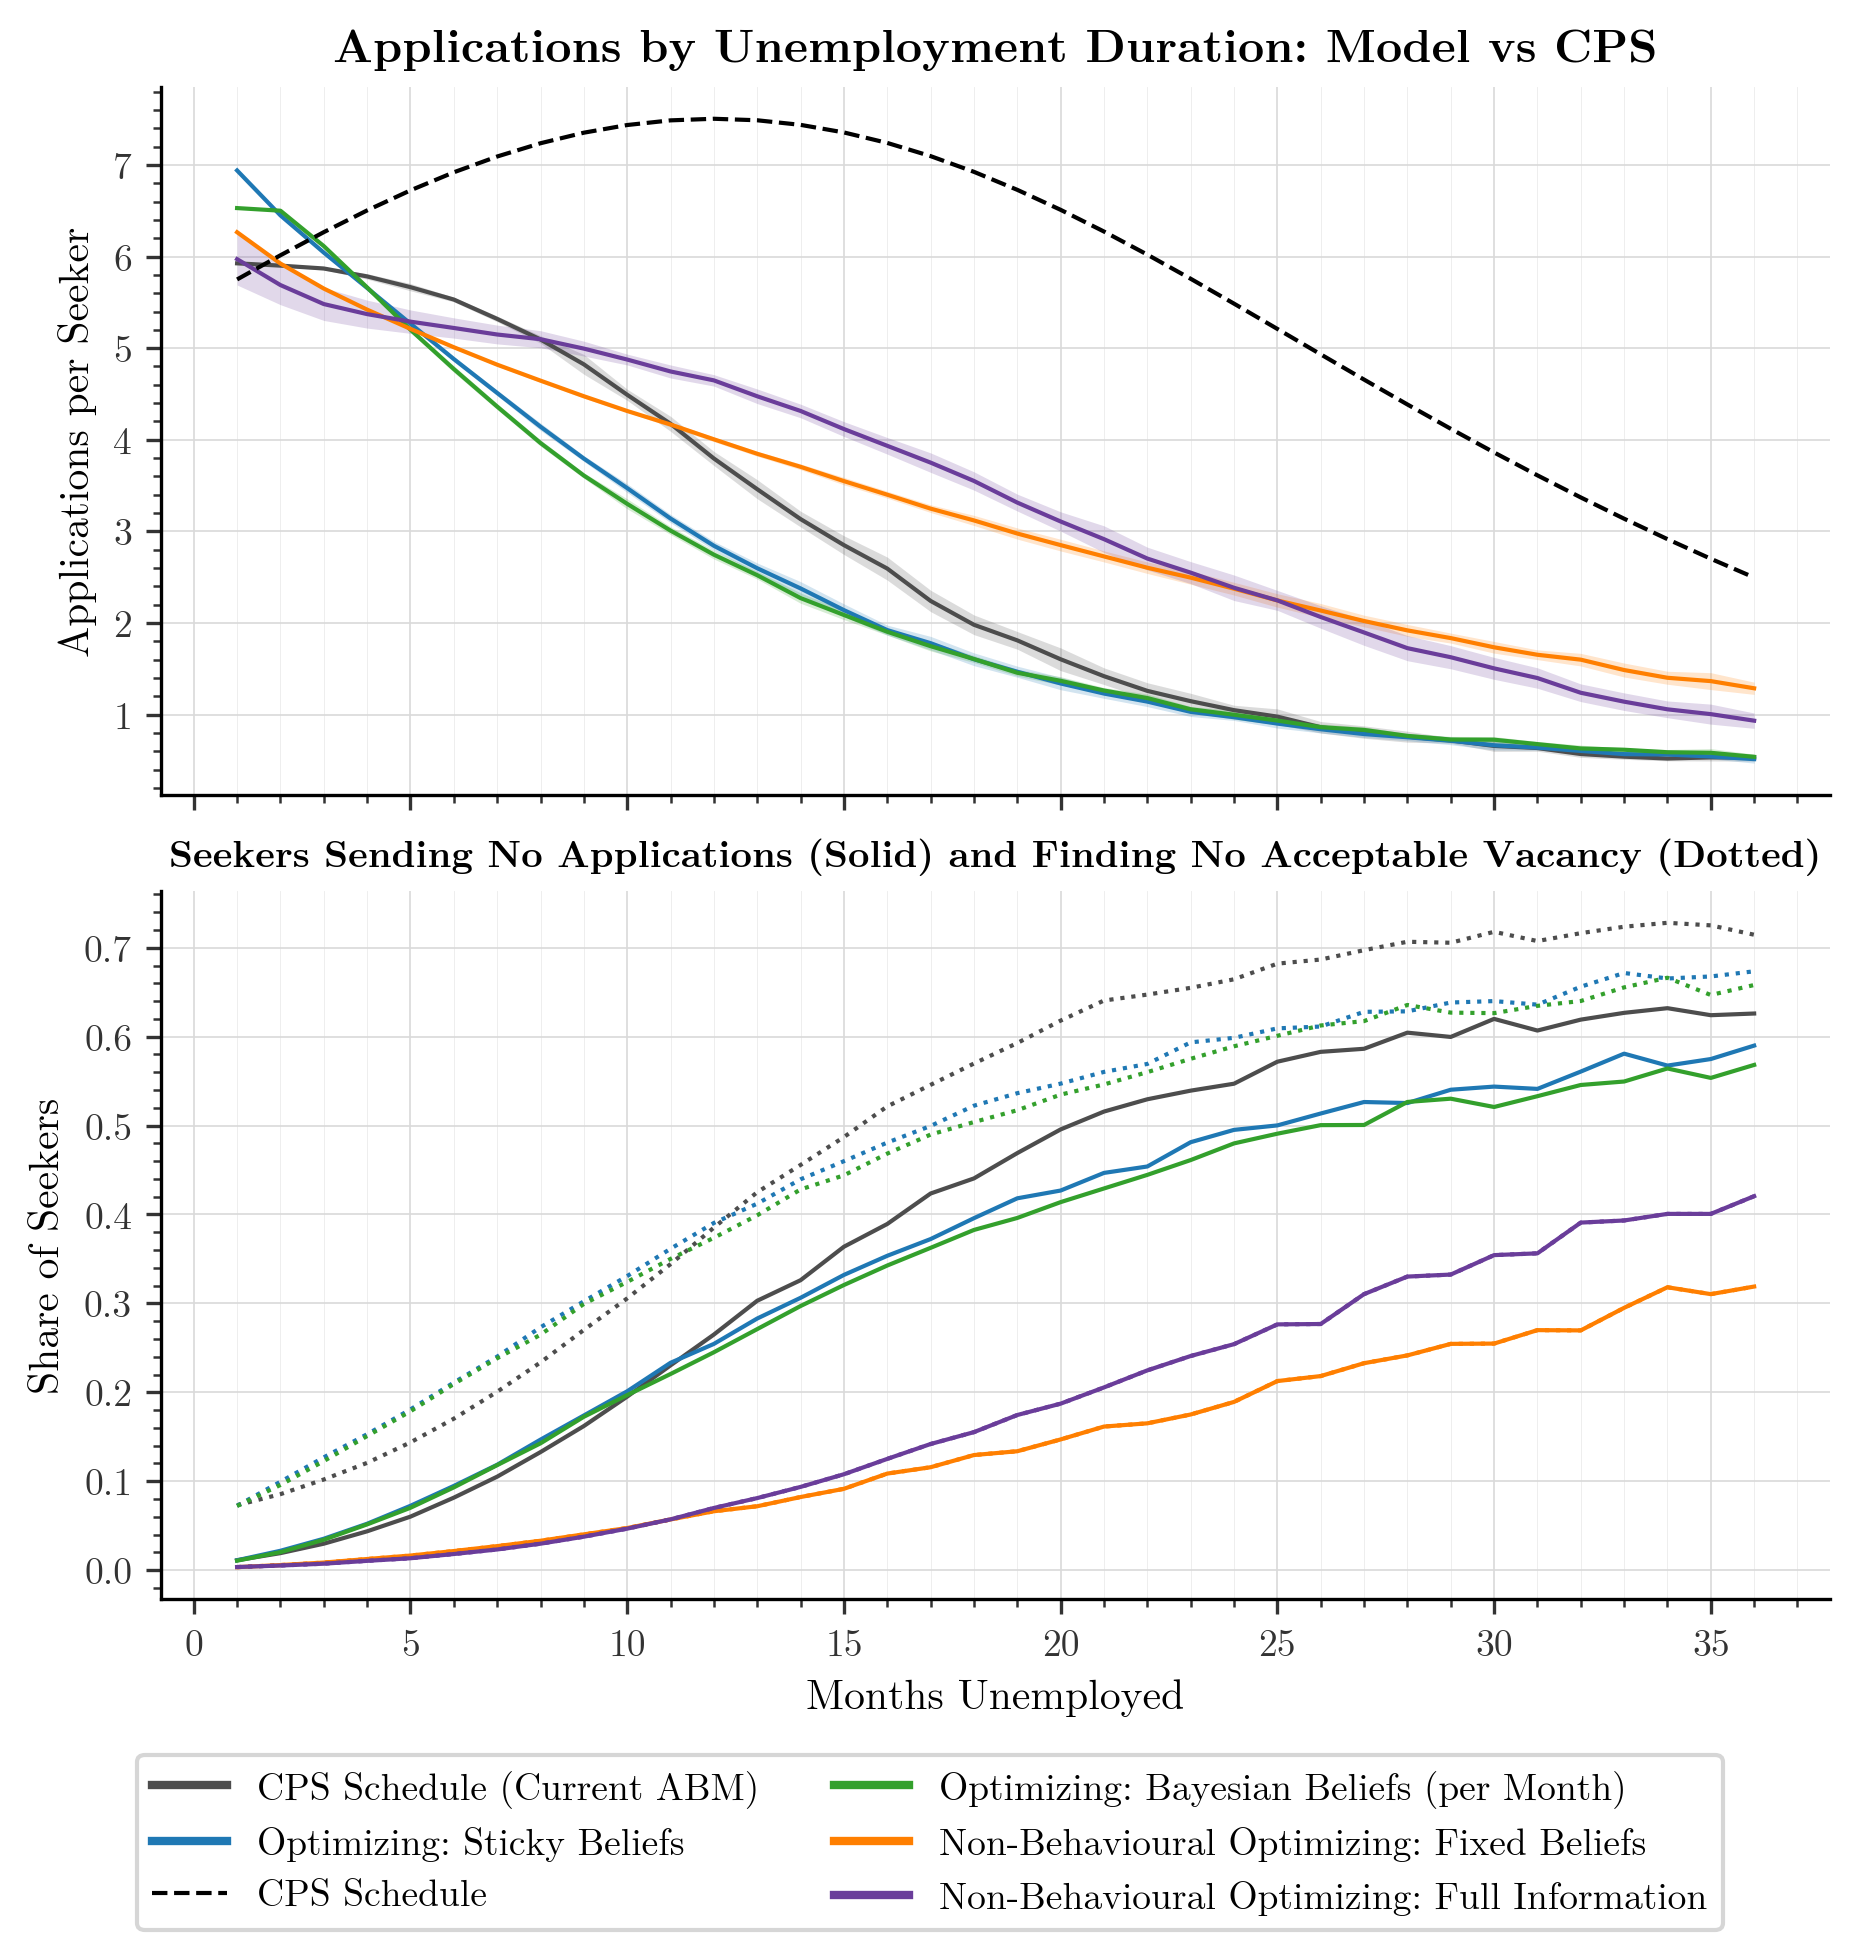
\includegraphics[width=\linewidth]{figures/applications_by_duration_vs_cps.png}
\caption{Realized applications by unemployment duration inside the ABM (top) and the share of seekers sending no
applications or finding no acceptable vacancy (bottom). Realized effort declines with duration under every rule,
including the baseline that draws effort from the CPS schedule. Long-duration seekers increasingly find no vacancy
above their reservation wage among the vacancies they can reach.}
\end{figure}

\bibliographystyle{apalike}
\begin{thebibliography}{}
\bibitem[Albrecht et~al., 2006]{albrecht2006equilibrium}
Albrecht, J., Gautier, P.~A., and Vroman, S. (2006). Equilibrium directed search with multiple applications.
\textit{Review of Economic Studies}, 73(4):869--891.
\bibitem[Burdett et~al., 2001]{burdett2001pricing}
Burdett, K., Shi, S., and Wright, R. (2001). Pricing and matching with frictions. \textit{Journal of Political
Economy}, 109(5):1060--1085.
\bibitem[Burdett and Vishwanath, 1988]{burdett1988declining}
Burdett, K. and Vishwanath, T. (1988). Declining reservation wages and learning. \textit{Review of Economic Studies},
55(4):655--665.
\bibitem[Chade and Smith, 2006]{chade2006simultaneous}
Chade, H. and Smith, L. (2006). Simultaneous search. \textit{Econometrica}, 74(5):1293--1307.
\bibitem[del Rio-Chanona et~al., 2021]{delriochanona2021occupational}
del Rio-Chanona, R.~M., Mealy, P., Beguerisse-D{\'i}az, M., Lafond, F., and Farmer, J.~D. (2021). Occupational
mobility and automation: A data-driven network model. \textit{Journal of the Royal Society Interface},
18(174):20200898.
\bibitem[Evans and Honkapohja, 2001]{evans2001learning}
Evans, G.~W. and Honkapohja, S. (2001). \textit{Learning and Expectations in Macroeconomics}. Princeton University
Press.
\bibitem[Galenianos and Kircher, 2009]{galenianos2009directed}
Galenianos, M. and Kircher, P. (2009). Directed search with multiple job applications. \textit{Journal of Economic
Theory}, 144(2):445--471.
\bibitem[Gonzalez and Shi, 2010]{gonzalez2010equilibrium}
Gonzalez, F.~M. and Shi, S. (2010). An equilibrium theory of learning, search, and wages. \textit{Econometrica},
78(2):509--537.
\bibitem[Kircher, 2009]{kircher2009efficiency}
Kircher, P. (2009). Efficiency of simultaneous search. \textit{Journal of Political Economy}, 117(5):861--913.
\bibitem[Krueger and Mueller, 2010]{krueger2010job}
Krueger, A.~B. and Mueller, A. (2010). Job search and unemployment insurance: New evidence from time use data.
\textit{Journal of Public Economics}, 94(3--4):298--307.
\bibitem[Krueger and Mueller, 2016]{krueger2016contribution}
Krueger, A.~B. and Mueller, A.~I. (2016). A contribution to the empirics of reservation wages. \textit{American
Economic Journal: Economic Policy}, 8(1):142--179.
\bibitem[Moen, 1997]{moen1997competitive}
Moen, E.~R. (1997). Competitive search equilibrium. \textit{Journal of Political Economy}, 105(2):385--411.
\bibitem[Mortensen, 1977]{mortensen1977unemployment}
Mortensen, D.~T. (1977). Unemployment insurance and job search decisions. \textit{Industrial and Labor Relations
Review}, 30(4):505--517.
\bibitem[Mueller et~al., 2021]{mueller2021job}
Mueller, A.~I., Spinnewijn, J., and Topa, G. (2021). Job seekers' perceptions and employment prospects:
Heterogeneity, duration dependence, and bias. \textit{American Economic Review}, 111(1):324--363.
\bibitem[Pissarides, 2000]{pissarides2000equilibrium}
Pissarides, C.~A. (2000). \textit{Equilibrium Unemployment Theory}. MIT Press, 2nd edition.
\bibitem[Spinnewijn, 2015]{spinnewijn2015unemployed}
Spinnewijn, J. (2015). Unemployed but optimistic: Optimal insurance design with biased beliefs. \textit{Journal of
the European Economic Association}, 13(1):130--167.
\bibitem[van~den Berg, 1990]{vandenberg1990nonstationarity}
van~den Berg, G.~J. (1990). Nonstationarity in job search theory. \textit{Review of Economic Studies}, 57(2):255--277.
\end{thebibliography}

\end{document}
